\documentclass[tikz,border=3pt]{standalone}
\usepackage{amsmath,amssymb}
\usetikzlibrary{arrows.meta,calc}
\definecolor{ink}{HTML}{203344}
\definecolor{blue}{HTML}{286389}
\definecolor{teal}{HTML}{147D80}
\definecolor{gold}{HTML}{A36A20}
\definecolor{muted}{HTML}{596873}
\begin{document}
% Research schematic; tiles and projection directions are not measured features.
% The three losses and detached normalization match models/visreg.py.
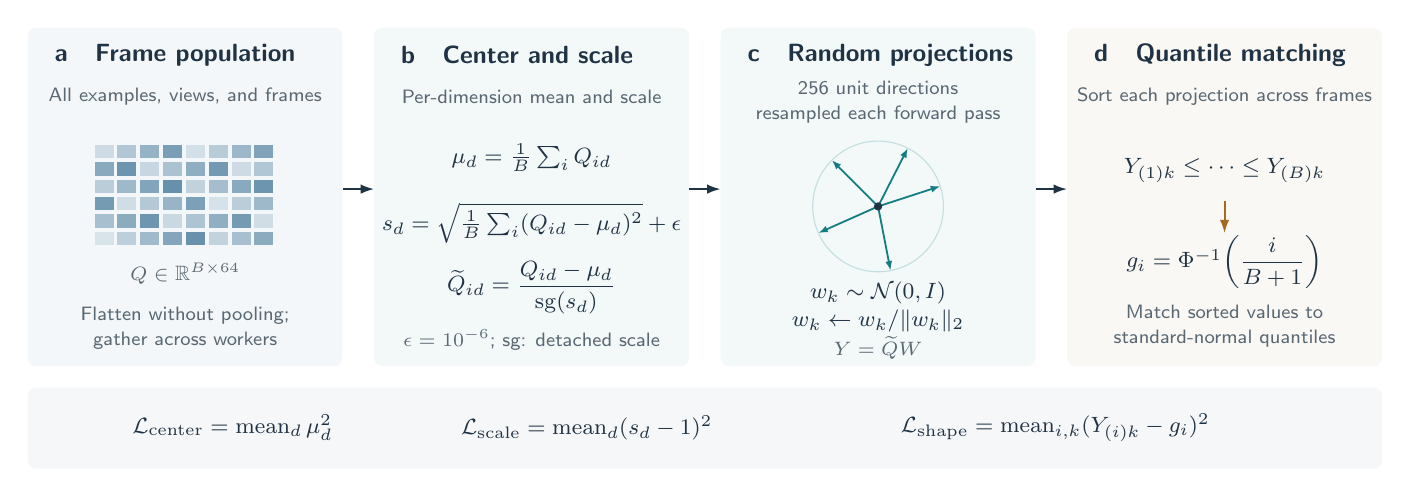
\begin{tikzpicture}[x=1cm,y=1cm,text=ink,
 font=\sffamily\fontsize{8}{10}\selectfont,
 head/.style={font=\sffamily\bfseries\fontsize{9}{11}\selectfont,anchor=west},
 small/.style={font=\sffamily\fontsize{7.5}{9}\selectfont,text=muted,align=center},
 flow/.style={-{Latex[length=1.7mm,width=1.2mm]},draw=ink,line width=.7pt}]
\path[use as bounding box] (0,0) rectangle (17.2,5.6);
\foreach \x/\col in {0/blue,4.4/teal,8.8/teal,13.2/gold}{
 \fill[\col!5,rounded corners=3pt] (\x,1.3) rectangle ++(4,4.3);
}
\node[head] at (.22,5.25) {a\quad Frame population};
\node[small] at (2,4.72) {All examples, views, and frames};
\foreach \i in {0,...,7}{\foreach \j in {0,...,5}{
 \pgfmathtruncatemacro{\shade}{18+mod(\i*13+\j*23,55)}
 \fill[blue!\shade] ({.85+\i*.29},{2.84+\j*.22}) rectangle ++(.24,.17);
}}
\node[small] at (2,2.48) {$Q\in\mathbb R^{B\times64}$};
\node[small] at (2,1.78) {Flatten without pooling;\\gather across workers};
\draw[flow] (4,3.55)--(4.4,3.55);
\node[head] at (4.62,5.25) {b\quad Center and scale};
\node[small] at (6.4,4.72) {Per-dimension mean and scale};
\node[align=center] at (6.4,3.95) {$\mu_d=\frac{1}{B}\sum_i Q_{id}$};
\node[align=center] at (6.4,3.12) {$s_d=\sqrt{\frac{1}{B}\sum_i(Q_{id}-\mu_d)^2}+\epsilon$};
\node[align=center] at (6.4,2.30) {$\widetilde Q_{id}=\dfrac{Q_{id}-\mu_d}{\operatorname{sg}(s_d)}$};
\node[small] at (6.4,1.64) {$\epsilon=10^{-6}$; sg: detached scale};
\draw[flow] (8.4,3.55)--(8.8,3.55);
\node[head] at (9.02,5.25) {c\quad Random projections};
\node[small] at (10.8,4.65) {256 unit directions\\resampled each forward pass};
\begin{scope}[shift={(10.8,3.33)}]
 \draw[teal!25] (0,0) circle (.83);
 \foreach \ang in {18,63,135,204,281}{\draw[-{Latex[length=1.2mm]},teal,line width=.65pt] (0,0)--(\ang:.83);}
 \fill[ink] (0,0) circle (1.5pt);
\end{scope}
\node[align=center] at (10.8,2.05) {$w_k\sim\mathcal N(0,I)$\\$w_k\leftarrow w_k/\|w_k\|_2$};
\node[small] at (10.8,1.53) {$Y=\widetilde Q W$};
\draw[flow] (12.8,3.55)--(13.2,3.55);
\node[head] at (13.42,5.25) {d\quad Quantile matching};
\node[small] at (15.2,4.72) {Sort each projection across frames};
\node[align=center] at (15.2,3.79) {$Y_{(1)k}\leq\cdots\leq Y_{(B)k}$};
\draw[flow,draw=gold] (15.2,3.40)--(15.2,2.99);
\node[align=center] at (15.2,2.62) {$g_i=\Phi^{-1}\!\left(\dfrac{i}{B+1}\right)$};
\node[small] at (15.2,1.81) {Match sorted values to\\standard-normal quantiles};
\fill[ink!4,rounded corners=3pt] (0,0) rectangle (17.2,1.03);
\node[align=center] at (2.6,.52) {$\mathcal L_{\rm center}=\operatorname{mean}_d\mu_d^2$};
\node[align=center] at (7.1,.52) {$\mathcal L_{\rm scale}=\operatorname{mean}_d(s_d-1)^2$};
\node[align=center] at (13.05,.52) {$\mathcal L_{\rm shape}=\operatorname{mean}_{i,k}(Y_{(i)k}-g_i)^2$};
\end{tikzpicture}
\end{document}
